\newenvironment{fragileframe}%
  {\begin{frame}[fragile,environment=fragileframe]}%
  {\end{frame}}

\section{Backgrounds}
\begin{fragileframe}
        \frametitle{Background Images}
        \framesubtitle{On Standard Frames}
        \begin{itemize}
      \item The next slide shows an image, embedded into the background of the frame layout.
      \item The background image is automatically cropped to the frame dimensions.
    \end{itemize}
        \begin{block}{How to install a background image}
        \tiny
        \begin{verbatim}
                \setbeamertemplate{background}{\includegraphics[width=\paperwidth]{background}}
                \begin{frame}
          Some text in front of the background image.
                \end{frame}
                \setbeamertemplate{background}{}
        \end{verbatim}
        \end{block}
\end{fragileframe}

\setbeamertemplate{background}{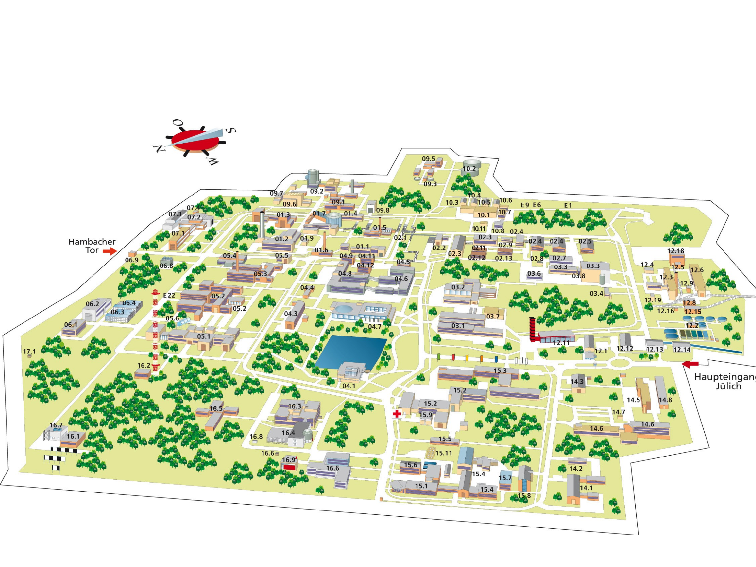
\includegraphics[width=\paperwidth]{lageplan}}
\begin{frame}
        \frametitle{Jülich Campus in the background}
        \vspace{5em}
        \centering
        \colorbox{fzjviolet}{\textcolor{fzjlightblue}{Some text in front of the background image.}}
\end{frame}
\setbeamertemplate{background}{}

\begin{fragileframe}
        \frametitle{Background Images}
        \framesubtitle{On Plain Frames}
        \begin{itemize}
          \item Use \verb!background canvas! instead of \verb!background! to flood fill a plain slide
          \item Again, the image is cropped to the frame boundaries
        \end{itemize}
        \begin{block}{How to install a background canvas image}
        \tiny
        \begin{verbatim}
                \setbeamertemplate{background canvas}{\includegraphics[width=\paperwidth]{background}}
                \begin{frame}[plain]
                \end{frame}
                \setbeamertemplate{background canvas}{}
        \end{verbatim}
        \end{block}
\end{fragileframe}

\setbeamertemplate{background canvas}{\includegraphics[width=\paperwidth]{background}}
\begin{frame}[plain]
\end{frame}
\setbeamertemplate{background canvas}{}

\begin{fragileframe}
        \begin{exampleblock}{Example Block}
                Just some text.
        \end{exampleblock}
        \begin{block}{Redefine commands with fancy colors}
                \verb+\renewcommand{\emph}[1]{\structure{#1}}+ \\
                Gives a nice blue text with every \verb+\emph{}+ command.
        \end{block}
\end{fragileframe}


\begin{comment}
\section{Split long text}
\begin{frame}[allowframebreaks,t]
        \frametitle{Automatically split long text}
        \framesubtitle{{\tt Beamer} can split text/lists to fit information on several
        slides}

        Lorem ipsum dolor sit amet, consetetur sadipscing elitr, sed diam nonumy eirmod
        tempor invidunt ut labore et dolore magna aliquyam erat, sed diam voluptua. At
        vero eos et accusam et justo duo dolores et ea rebum. Stet clita kasd gubergren,
        no sea takimata sanctus est Lorem ipsum dolor sit amet. Lorem ipsum dolor sit
        amet, consetetur sadipscing elitr, sed diam nonumy eirmod tempor invidunt ut
        labore et dolore magna aliquyam erat, sed diam voluptua. At vero eos et accusam
        et justo duo dolores et ea rebum. Stet clita kasd gubergren, no sea takimata
        sanctus est Lorem ipsum dolor sit amet. Lorem ipsum dolor sit amet, consetetur
        sadipscing elitr, sed diam nonumy eirmod tempor invidunt ut labore et dolore
        magna aliquyam erat, sed diam voluptua. At vero eos et accusam et justo duo
        dolores et ea rebum. Stet clita kasd gubergren, no sea takimata sanctus est Lorem
        ipsum dolor sit amet.

        Duis autem vel eum iriure dolor in hendrerit in vulputate velit esse molestie
        consequat, vel illum dolore eu feugiat nulla facilisis at vero eros et accumsan
        et iusto odio dignissim qui blandit praesent luptatum zzril delenit augue duis
        dolore te feugait nulla facilisi. Lorem ipsum dolor sit amet, consectetuer
        adipiscing elit, sed diam nonummy nibh euismod tincidunt ut laoreet dolore magna
        aliquam erat volutpat.

        Ut wisi enim ad minim veniam, quis nostrud exerci tation ullamcorper suscipit
        lobortis nisl ut aliquip ex ea commodo consequat. Duis autem vel eum iriure dolor
        in hendrerit in vulputate velit esse molestie consequat, vel illum dolore eu
        feugiat nulla facilisis at vero eros et accumsan et iusto odio dignissim qui
        blandit praesent luptatum zzril delenit augue duis dolore te feugait nulla
        facilisi.
\end{frame}
\end{comment}
